
\blank
\newpage

\section{Neural Language Models}

    \subsection{Recurrent Neural Networks (RNN)}
            
    
        Le \textbf{Reti Neurali Ricorrenti} (Recurrent Neural Networks - RNN) nascono per gestire la natura intrinsecamente sequenziale del linguaggio. A differenza dei modelli a finestra fissa (sliding windows), le RNN elaborano l'input un elemento alla volta, mantenendo una "memoria" di ciò che hanno visto in precedenza.
    
        Il modello base, introdotto da Elman nel 1990, introduce il concetto di \textbf{stato nascosto} (hidden state) che evolve nel tempo.
        Al passo temporale $t$, la rete riceve in input il token corrente $x_t$ e lo stato nascosto del passo precedente $h_{t-1}$.
        
        \begin{figure}[H]
            \centering
            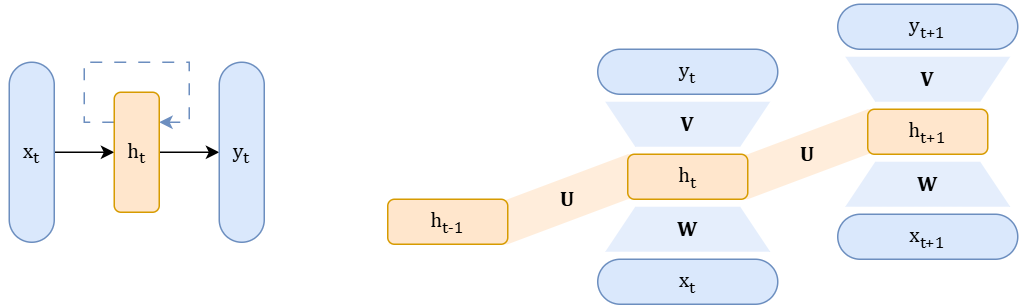
\includegraphics[width=0.8\linewidth]{imgs/schema_6_1.png}
            \label{fig:fig61}
        \end{figure}

        Le equazioni fondamentali per l'aggiornamento dello stato e il calcolo dell'output sono:
        
        $$
            h_t = g(U h_{t-1} + W x_t),\qquad
            y_t = f(V h_t)
        $$
        
        Dove:
        \begin{itemize}
            \item $U, W, V$ sono le matrici dei pesi (condivise per tutti i passi temporali).
            \item $g$ è la funzione di attivazione (solitamente $tanh$ o ReLU).
            \item $f$ è la funzione di output (es. $softmax$ per la classificazione).
        \end{itemize}
        
        La rete può essere "srotolata" (unrolled) nel tempo, trasformandola in una lunga catena di reti feed-forward che condividono gli stessi pesi (perciò la rete non è iterata dentro se stessa, ma interconnessa ad altre reti). Questo permette di utilizzare l'algoritmo di \textbf{Backpropagation Through Time (BPTT)} per l'addestramento.
    
    \newpage

    \subsubsection{LSTM}
        
        Le RNN classiche (o "vanilla") soffrono del problema del \textbf{Vanishing Gradient} (evanescenza del gradiente). 
        Quando si calcola l'errore e lo si propaga indietro nel tempo per molti passi, il gradiente tende a diventare piccolissimo, impedendo alla rete di imparare dipendenze a lungo; inoltre l'onero computazionali è elevato.\\

        Per risolvere questo problema sono state introdotte le \textbf{Long Short-Term Memory (LSTM)}. Le LSTM introducono una "cella di memoria" ($c_t$) separata dallo stato nascosto ($h_t$) e utilizzano dei \textbf{gate} (porte) per controllare il flusso di informazioni:
                    
        \begin{figure}[H]
            \centering
            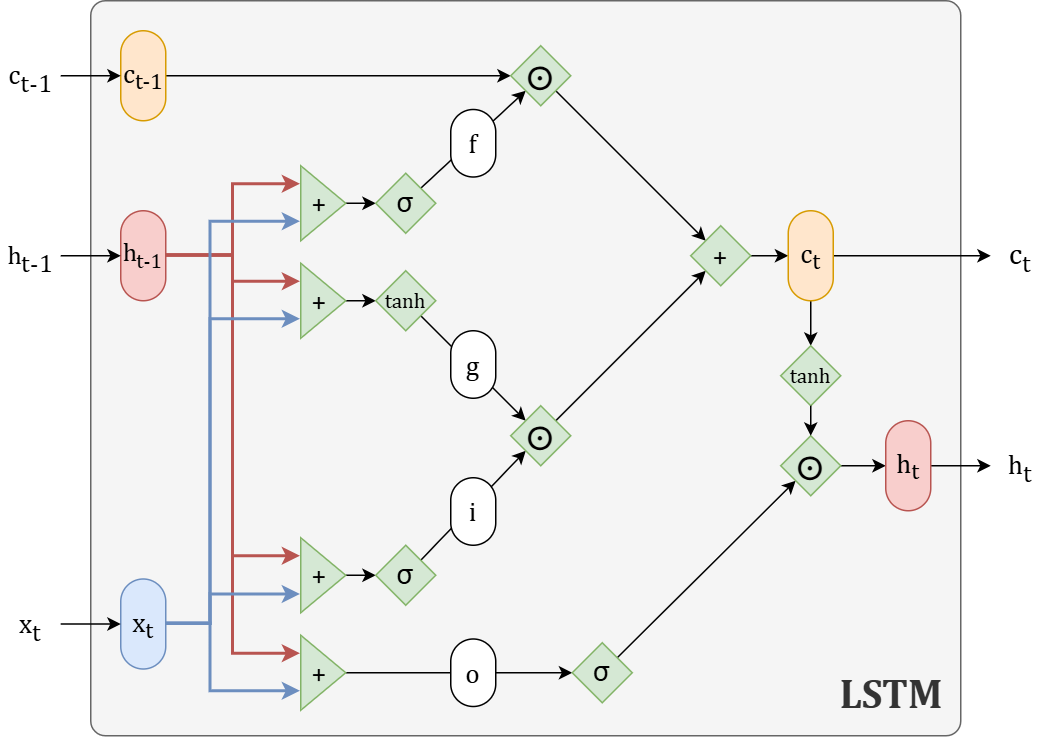
\includegraphics[width=0.8\linewidth]{imgs/schema_6_2.png}
            \label{fig:fig62}
        \end{figure}

        \begin{itemize}
        
            \item \textbf{Forget Gate ($f_t$)}: Decide quali informazioni dimenticare dallo stato precedente.
            \[ f_t = \sigma(U_f h_{t-1} + W_f x_t) \]
            
            \item \textbf{Input Gate ($i_t$) e Candidate ($g_t$)}: Decidono quali nuove informazioni memorizzare.
            \[ i_t = \sigma(U_i h_{t-1} + W_i x_t), \qquad
            g_t = \tanh(U_g h_{t-1} + W_g x_t) \]
            
            \item \textbf{Update della Cella ($c_t$)}: Combina la memoria vecchia (filtrata) con quella nuova.
            \[ c_t = f_t \odot c_{t-1} + i_t \odot g_t \]
            
            \item \textbf{Output Gate ($o_t$)}: Decide cosa esporre come output (stato nascosto).
            \[ o_t = \sigma(U_o h_{t-1} + W_o x_t), \qquad
            h_t = o_t \odot \tanh(c_t) \]
            
        \end{itemize}

    \newpage
    
    \subsubsection{Advanced Architectures}
    
        Per migliorare le capacità rappresentative delle RNN, sono state introdotte due varianti architetturali fondamentali che spesso vengono combinate tra loro.

        \begin{wrapfigure}{r}{0.4\textwidth}
            \vspace{-15pt}
            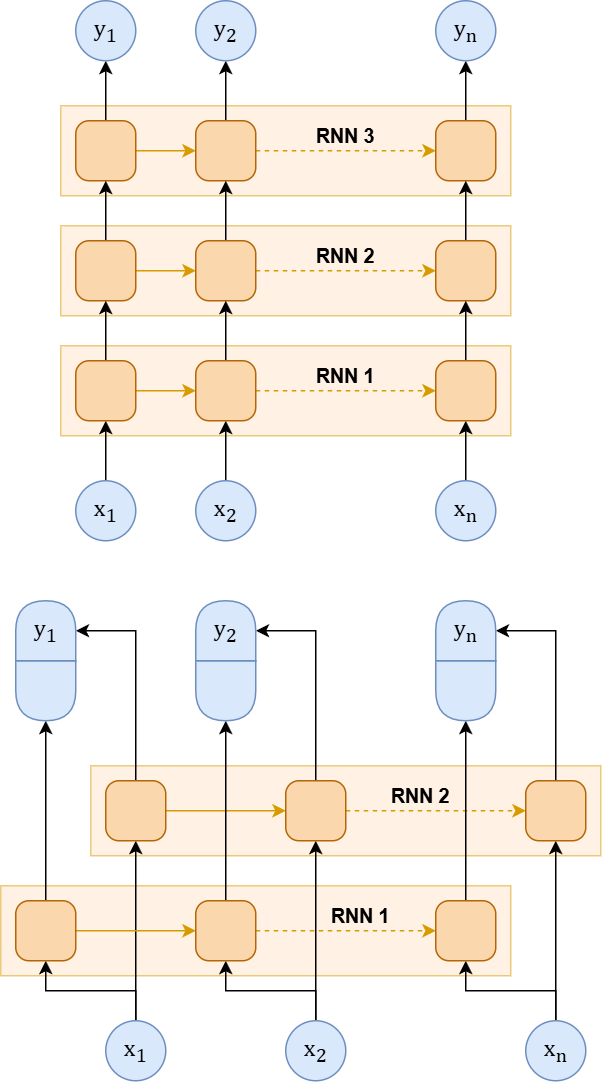
\includegraphics[width=1\linewidth]{imgs/schema_6_3.png}
            \label{fig:fig63}
        \end{wrapfigure}

        \paragraph{Stacked RNN (Reti Impilate)}
        In una Stacked RNN, più strati ricorrenti vengono impilati uno sopra l'altro. L'output (o la sequenza degli stati nascosti) del layer $l$ al tempo $t$ diventa l'input per il layer $l+1$ allo stesso istante temporale $t$.
        Questo permette alla rete di apprendere rappresentazioni gerarchiche più complesse: i layer inferiori tendono a catturare caratteristiche sintattiche o locali, mentre i layer superiori possono catturare concetti semantici più astratti.

        \paragraph{Bidirectional RNN (Reti Bidirezionali)}
        Le RNN standard elaborano l'input solo in avanti (dal passato al futuro). Tuttavia, in molti task l'intera frase è disponibile fin dall'inizio ed è utile conoscere anche il contesto futuro.
        
        Le \textbf{Bi-RNN} sono composte da due reti indipendenti che operano sulla stessa sequenza:
        
        \begin{itemize}
            
            \item Una \textbf{Forward RNN} che legge la sequenza da sinistra a destra: 
            $$\overrightarrow{h}_t = RNN_{fwd}(x_1, \dots, x_t)$$
            
            \item Una \textbf{Backward RNN} che legge la sequenza da destra a sinistra: 
            $$\overleftarrow{h}_t = RNN_{bwd}(x_n, \dots, x_t)$$
            
        \end{itemize}
        
        L'output finale al passo $t$ è solitamente la concatenazione dei due stati nascosti:
        \[ h_t = [\overrightarrow{h}_t \oplus \overleftarrow{h}_t] \]
    
    \subsubsection{Encoder-Decoder Architecture (Seq2Seq)}
    
        Per task come la traduzione automatica, dove la lunghezza dell'input differisce da quella dell'output, si utilizza l'architettura \textbf{Encoder-Decoder}:
        
        \begin{enumerate}
        
            \item \textbf{Encoder}: Una RNN legge tutta la frase di input e la comprime in un unico vettore finale chiamato \textit{Context Vector} ($c$).
            
            \item \textbf{Decoder}: Un'altra RNN prende questo vettore $c$ e genera la frase di output, parola per parola.
        
        \end{enumerate}

        \begin{figure}[H]
            \centering
            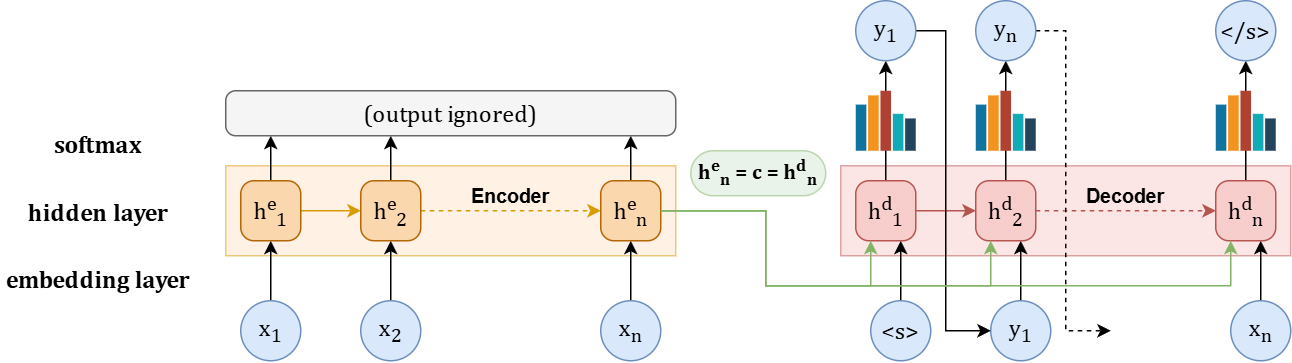
\includegraphics[width=0.8\linewidth]{imgs/schema_6_5.png}
            \label{fig:fig65}
        \end{figure}
        
        Il limite principale di questo approccio è il \textbf{Collo di Bottiglia (Bottleneck)}: costringere tutta l'informazione di una frase lunga in un unico vettore di dimensione fissa $c$ causa perdita di informazioni.

    \newpage
    
    \subsection{Attention}
    
    Per superare il problema del "collo di bottiglia", è stato introdotto il meccanismo di \textbf{Attenzione} L'idea chiave è che il Decoder non dovrebbe basarsi solo su un unico vettore statico, ma dovrebbe poter "guardare" (attendere) a tutti gli stati nascosti dell'Encoder a ogni passo di generazione.
    
    \subsubsection{Funzionamento}
    
        Ad ogni passo $i$ del Decoder, si calcola un nuovo vettore di contesto $c_i$ specifico per quel momento:
        
        \begin{figure}[H]
            \centering
            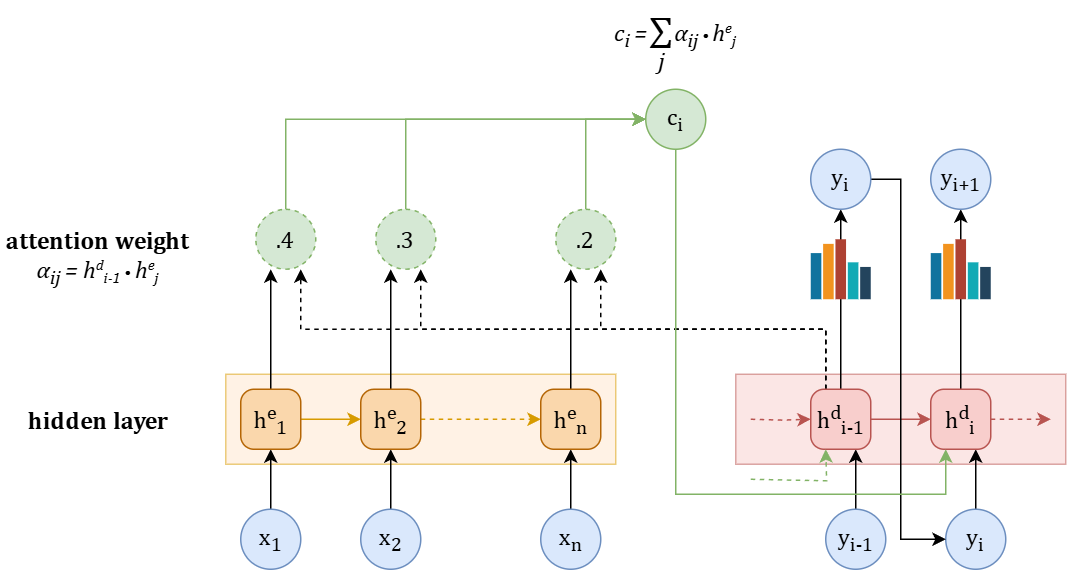
\includegraphics[width=0.8\linewidth]{imgs/schema_6_6.png}
            \label{fig:fig66}
        \end{figure}
        
        \begin{enumerate}
            \item Si calcola uno \textbf{score} di similarità tra lo stato attuale del Decoder ($h_{i-1}^d$) e tutti gli stati dell'Encoder ($h_j^e$). Lo score più semplice è il prodotto scalare (Dot-Product):
            \[ score(h_{i-1}^d, h_j^e) = h_{i-1}^d \cdot h_j^e \]
            Oppure con pesi addestrabili (Attention generalizzata):
            \[ score(h_{i-1}^d, h_j^e) = (h_{i-1}^d)^T W_s h_j^e \]
            
            \item Si normalizzano gli score tramite una funzione \textbf{Softmax} per ottenere i pesi di attenzione $\alpha_{ij}$ (che sommano a 1):
            \[ \alpha_{ij} = \frac{\exp(score(h_{i-1}^d, h_j^e))}{\sum_k \exp(score(h_{i-1}^d, h_k^e))} \]
            
            \item Si calcola il vettore di contesto come somma pesata degli stati dell'encoder:
            \[ c_i = \sum_j \alpha_{ij} h_j^e \]
        \end{enumerate}
        
        In questo modo, il modello può concentrarsi ("prestare attenzione") sulla parola rilevante della frase sorgente mentre genera la traduzione corrispondente.
    
    \newpage

    \subsection{Transformers}
    
        Nel 2017, il paper \textit{"Attention Is All You Need"} (Vaswani et al., Google Brain) ha introdotto l'architettura Transformer, che ha rivoluzionato il NLP. A differenza delle RNN, i Transformer non processano i dati sequenzialmente ma in parallelo, basandosi interamente sul meccanismo di attenzione.\\
        
        \textit{Fare attenzione secondo certi criteri funge da strategie per selezionare i coefficienti che realmente devo guardare nella matrice.}
        
        \begin{figure}[H]
            \centering
            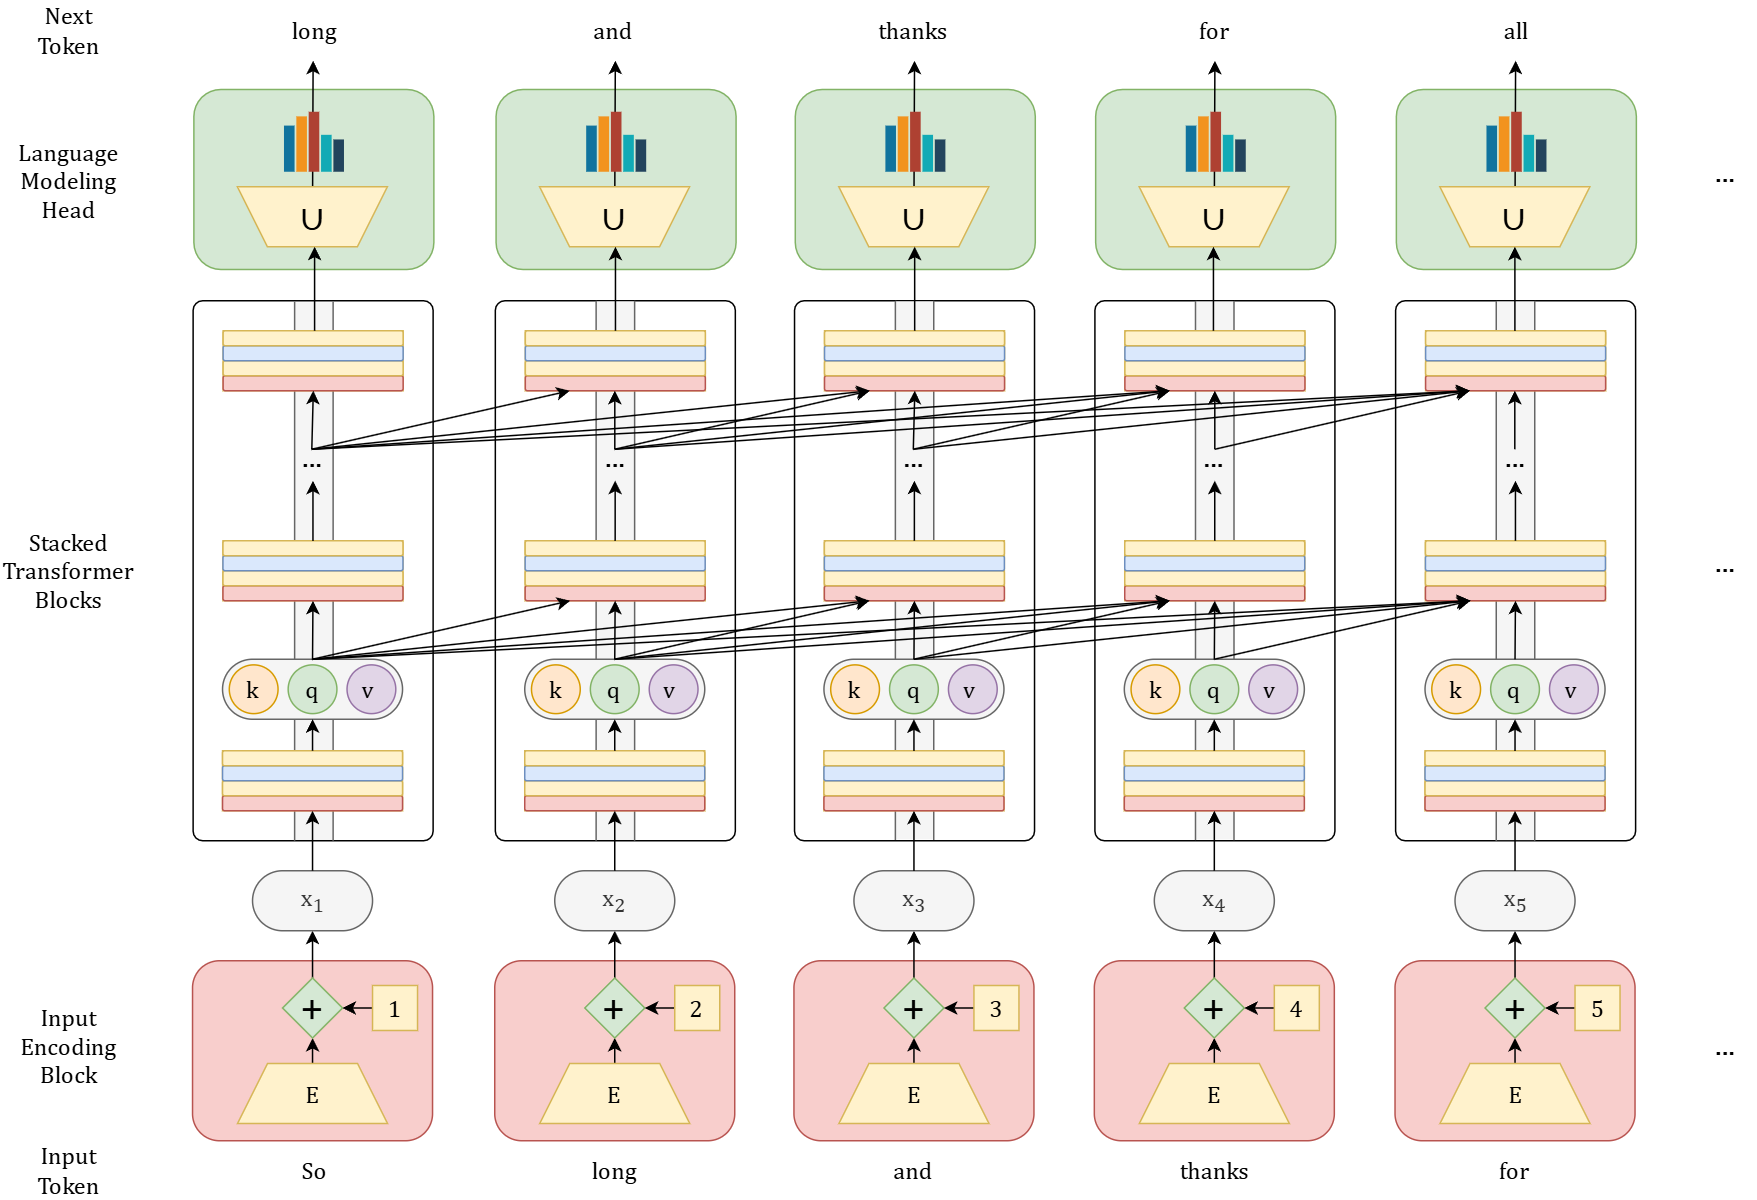
\includegraphics[width=1\linewidth]{imgs/schema_6_7.png}
            \label{fig:fig67}
        \end{figure}

        \subsubsection{Dagli Embedding Statici a quelli Contestuali}

            I modelli precedenti (come Word2Vec) generavano \textbf{embedding statici}: una parola aveva sempre la stessa rappresentazione vettoriale indipendentemente dal contesto.
            Consideriamo l'esempio:
            \begin{quote}
                \textit{"The chicken didn't cross the road because \textbf{it} was too tired."}\\
                \textit{"The chicken didn't cross the road because \textbf{it} was too wide."}
            \end{quote}
            Negli embedding statici, il vettore per "it" è identico in entrambe le frasi. Tuttavia, nel primo caso "it" si riferisce al pollo (chicken), nel secondo alla strada (road).
            
            Il Transformer introduce gli \textbf{Embedding Contestuali}: la rappresentazione di una parola viene costruita integrando le informazioni delle parole che la circondano. Ogni parola "presta attenzione" (Self-Attention) ai vicini rilevanti per disambiguare il proprio significato.
        
        \newpage

        \subsubsection{Il Meccanismo di Self-Attention}

            \begin{wrapfigure}{r}{0.45\textwidth}
                \vspace{-15pt}
                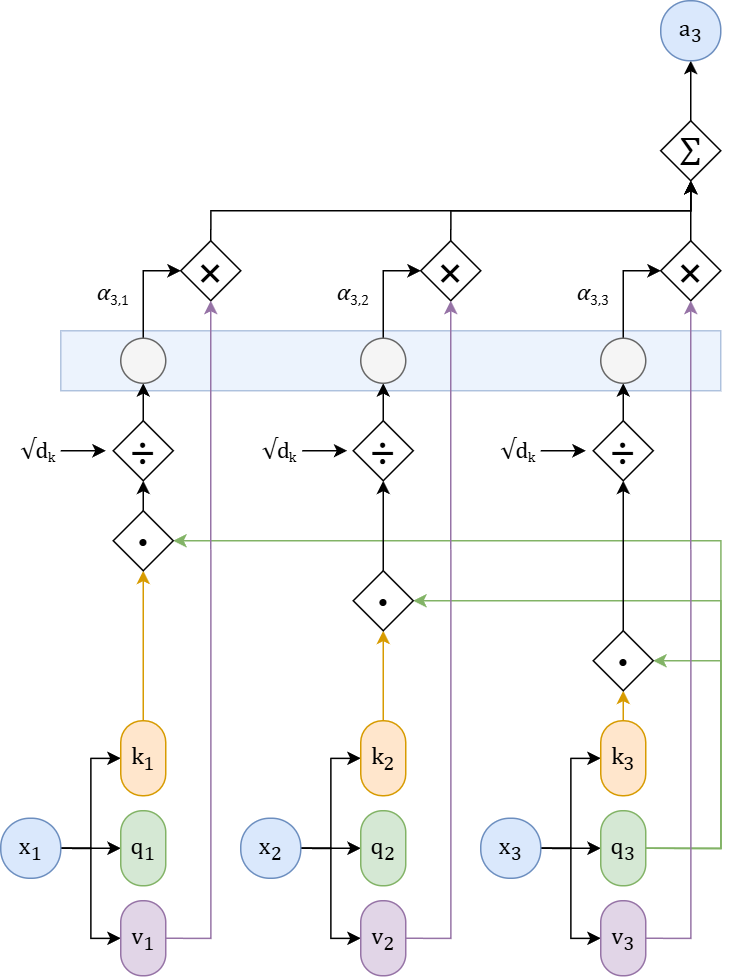
\includegraphics[width=1\linewidth]{imgs/schema_6_8.png}
                \label{fig:fig68}
            \end{wrapfigure}

            L'attenzione è formalmente un metodo per eseguire una somma pesata di vettori. Nel Transformer, ogni token di input $x_i$ viene proiettato in tre vettori distinti tramite matrici di pesi addestrabili ($W^Q, W^K, W^V$):
            
            \begin{itemize}
                \item \textbf{Query ($q_i = x_i W^Q$)}: Rappresenta il token corrente che "cerca" informazioni.
                \item \textbf{Key ($k_i = x_i W^K$)}: Rappresenta il token come "etichetta" per essere trovato.
                \item \textbf{Value ($v_i = x_i W^V$)}: Contiene il contenuto informativo effettivo del token.
            \end{itemize}
            
            \paragraph{Calcolo dello Score e dell'Output}
            Per calcolare quanto il token $i$ deve prestare attenzione al token $j$, si calcola il prodotto scalare tra la Query di $i$ e la Key di $j$. Questo valore viene scalato per la radice quadrata della dimensione delle key ($d_k$) per evitare gradienti instabili:
            \[ score(x_i, x_j) = \frac{q_i \cdot k_j}{\sqrt{d_k}} \]
            
            Successivamente si applica la Softmax per ottenere i pesi di attenzione $\alpha_{ij}$ (che sommano a 1):
            \[ \alpha_{ij} = \text{softmax}\left( \frac{q_i \cdot k_j}{\sqrt{d_k}} \right) \]
            
            L'output $a_i$ per il token $i$ è la somma pesata dei vettori Value degli altri token:
            \[ a_i = \sum_{j} \alpha_{ij} v_j \]
            
            \paragraph{Formulazione Matriciale}
            Operando su tutti i token contemporaneamente (impacchettati in una matrice $X$), il calcolo diventa altamente parallelizzabile:
            \[ Attention(Q, K, V) = \text{softmax}\left( \frac{QK^T}{\sqrt{d_k}} \right) V \]
        
        \subsubsection{Multi-Head Attention}
            
        Invece di avere una singola testa di attenzione, il Transformer ne usa molteplici ($h$ heads). Ogni testa ha le proprie matrici indipendenti $W^Q_c, W^K_c, W^V_c$.
            L'intuizione è che diverse teste possono focalizzarsi su relazioni linguistiche diverse (es. una testa lega soggetto-verbo, un'altra aggettivo-sostantivo).
            Gli output delle teste vengono concatenati e proiettati linearmente tramite una matrice $W^O$:
            \[ MultiHead(X) = [head_1 \oplus head_2 \dots \oplus head_h] W^O \]
        
        \subsubsection{Mascheramento (Masking)}
            
            Nel contesto del Language Modeling (predire la parola successiva), il modello non deve "vedere nel futuro". Durante il calcolo dell'attenzione $QK^T$, si applica una maschera che imposta a $-\infty$ gli score relativi ai token futuri (triangolo superiore della matrice).
            Dopo la softmax, questi valori diventano $0$, impedendo il flusso di informazioni dal futuro.
            \[ A = \text{softmax}\left( \text{mask}\left( \frac{QK^T}{\sqrt{d_k}} \right) \right) V \]
        
        \newpage

        \subsubsection{Il Blocco Transformer}

            \begin{wrapfigure}{r}{0.2\textwidth}
                \vspace{-15pt}
                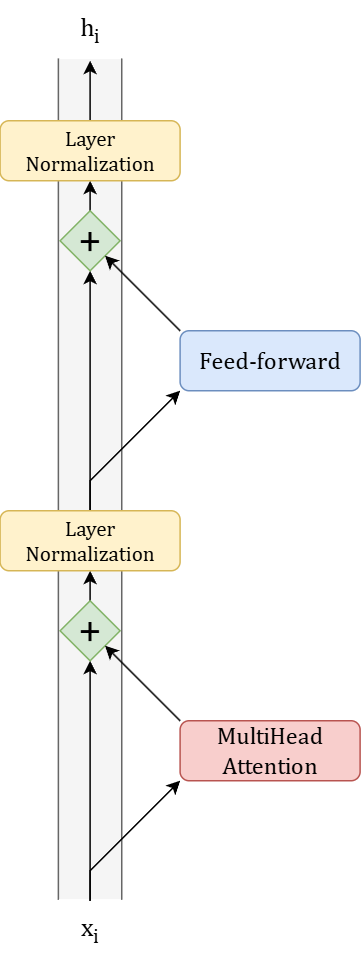
\includegraphics[width=1\linewidth]{imgs/schema_6_9.png}
                \label{fig:fig69}
            \end{wrapfigure}

            Un blocco Transformer completo è composto da diversi sotto-strati, uniti da connessioni residuali (Residual Connections) e normalizzazione.
            Il flusso per un token $x_i$ attraverso un blocco è:
            
            \begin{enumerate}
                \item \textbf{Multi-Head Attention}: Elabora il contesto.
                \item \textbf{Add \& Norm}: Si somma l'input originale all'output dell'attenzione (connessione residua) e si applica la \textbf{Layer Normalization}.
                \[ t^1 = \text{MHA}(x); \quad t^2 = \text{LayerNorm}(x + t^1) \]
                \item \textbf{Feed Forward Network (FFN)}: Una rete neurale dense applicata a ogni token indipendentemente, che introduce non-linearità.
                \[ FFN(x) = \text{ReLU}(x W_1 + b_1) W_2 + b_2 \]
                \item \textbf{Add \& Norm}: Un'altra connessione residua seguita da normalizzazione.
                \[ output = \text{LayerNorm}(t^2 + FFN(t^2)) \]
            \end{enumerate}
            
            \textbf{Nota sul Residual Stream:} I vettori scorrono attraverso la rete lungo un "flusso residuo". I layer di attenzione leggono da questo flusso e scrivono (sommano) nuove informazioni, arricchendo progressivamente la rappresentazione del token.
        
        \subsubsection{Input: Token e Position Embeddings}
            
            Poiché l'attenzione è invariante all'ordine (tratta le parole come un "sacchetto"), è necessario iniettare esplicitamente l'informazione posizionale.
            L'input finale del Transformer è la somma di due embedding:
            
            \[ X = \text{TokenEmbedding} + \text{PositionEmbedding} \]
            
            \begin{itemize}
                \item \textbf{Token Embedding}: Matrice $E$ di dimensione $|V| \times d$.
                \item \textbf{Position Embedding}: In particolare l'approccio dei \textit{Learned Position Embeddings}, si apprende una matrice dove ogni riga rappresenta una posizione assoluta (1, 2, 3...) fino a una lunghezza massima $N$.
            \end{itemize}
            
        \subsubsection{Output: La Language Modeling Head}
        
            Alla fine degli stack di blocchi Transformer, abbiamo un vettore $h_N^L$ per l'ultimo token, che rappresenta il suo significato contestualizzato. Per predire la parola successiva:
            
            \begin{enumerate}
                \item Si usa un \textbf{Unembedding Layer} (spesso è la trasposta della matrice di embedding $E^T$, tecnica nota come \textit{Weight Tying}). Questo proietta il vettore dalla dimensione del modello $d$ a quella del vocabolario $|V|$.
                \item Si ottengono i \textbf{Logits} ($u$).
                \item Si applica la \textbf{Softmax} per ottenere una distribuzione di probabilità su tutto il vocabolario.
            \end{enumerate}
            $$P(w_{next}) = \text{softmax}(h_N^L E^T)$$
            
            Da questa distribuzione si campiona il token successivo.